% ----- Consignes exo 2 ----- %
\begin{td-exo}[Combinaison convexe]\, % 2
	\begin{enumerate}
		\item Rappeler la définition d'une combinaison convexe.
		\item Est-ce que le point \(A\) de coordonnées \((1,1,1)\) est une combinaison convexe
		des points \((2,2,0), (0,0,3), (0,0,0)\)?
		\item Déterminer si le point de coordonnées \((0,7)\) est une combinaison convexe
		des points \((3,6),(-6,9),(2,1),(-1,1)\).
		\item Déterminer graphiquement si le point de coordonnées \((1,2)\) est une combinaison
		convexe des points \((1,1)\) et \((2,-1)\).
	\end{enumerate}
\end{td-exo}

% ----- Solutions exo 2 ----- %
\iftoggle{showsolutions}{
	\begin{td-sol}[]\ %
		\begin{enumerate}
			\item Une combinaison convexe de points \(x_1, x_2, \ldots, x_k\) est une combinaison
			\begin{equation*}
				\sum_{i=1}^k \lambda_i x_i
			\end{equation*}
			avec \(\lambda_i \geq 0\) et \(\sum_{i=1}^k \lambda_i = 1\).

			\item On cherche \(\lambda_1, \lambda_2, \lambda_3 \geq 0\) tels que
			\begin{equation*}
				\lambda_1 (2,2,0) + \lambda_2 (0,0,3) + \lambda_3 (0,0,0) = (1,1,1).
			\end{equation*}
			Ici on voit que \((\lambda1, \lambda_2, \lambda_3) = (0.5, 1/3, 0)\) est une solution.

			\item On cherche \(\lambda_1, \lambda_2, \lambda_3, \lambda_4 \geq 0\) tels que
			\begin{equation*}
				\lambda_1 (3,6) + \lambda_2 (-6,9) + \lambda_3 (2,1) + \lambda_4 (-1,1) = (0,7).
			\end{equation*}
			Cela revient à résoudre le système suivant:
			\begin{equation*}
				\begin{cases}
					3\lambda_1 - 6\lambda_2 + 2\lambda_3 - \lambda_4 = 0 \\
					6\lambda_1 + 9\lambda_2 + \lambda_3 + \lambda_4 = 7 \\
					\lambda_1 + \lambda_2 + \lambda_3 + \lambda_4 = 1
				\end{cases}
			\end{equation*}
			En résolvant on obtient la famille de solutions:
			\begin{equation*}
				\lambda_1 = \frac t2 + \frac 23,\quad
				\lambda_2 = \frac 13 + \frac {5t}{16},\quad
				\lambda_3 = \frac{-19t}{16},\quad
				\lambda_4 = t
			\end{equation*}
			avec \(t\in\bb R\). En imposant \(\lambda_i \geq 0\) on trouve \(t=0\) et donc
			\((\lambda_1, \lambda_2, \lambda_3, \lambda_4) = (2/3, 1/3, 0, 0)\).

			\item Graphiquement, on voit que le point \((1,2)\) n'est pas sur le segment
			entre les points \((1,1)\) et \((2,-1)\). Donc ce n'est pas une combinaison convexe:

			\begin{center}
				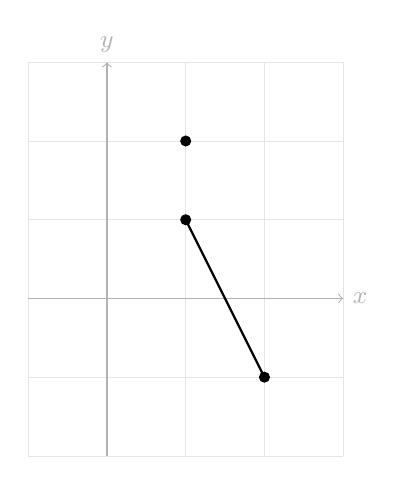
\begin{tikzpicture}[scale=1, font=\small]
					% coordinates
					\coordinate (A) at (1,1);
					\coordinate (B) at (2,-1);
					\coordinate (P) at (1,2);

					% light grid
					\draw[step=1cm, very thin, gray!20] (-1,-2) grid (3,3);

					% axes
					\draw[->, thin, gray!60] (-1,0) -- (3,0) node[right] {\(x\)};
					\draw[->, thin, gray!60] (0,-2) -- (0,3) node[above] {\(y\)};

					% segment AB
					\draw[thick] (A) -- (B) node[midway, below right=1pt] {};

					% points
					\fill (A) circle (2pt) node[below left=2pt] {};
					\fill (B) circle (2pt) node[below right=2pt] {};
					\fill (P) circle (2pt) node[above left=2pt] {};
				\end{tikzpicture}
			\end{center}
		\end{enumerate}
	\end{td-sol}
}{}

